%---------------Consultar Citas Paciente-------------

\subsection{IU3 Consultar Citas del paciente}

\subsubsection{Objetivo}
Mostrar al paciente la información de las citas que ha agendado en la clínica.

\subsubsection{Diseño}
Esta pantalla aparece al presionar el botón ``Consultar mis citas'' en la pantalla de inicio del Paciente.

\begin{figure}[htbp!]
	\centering
	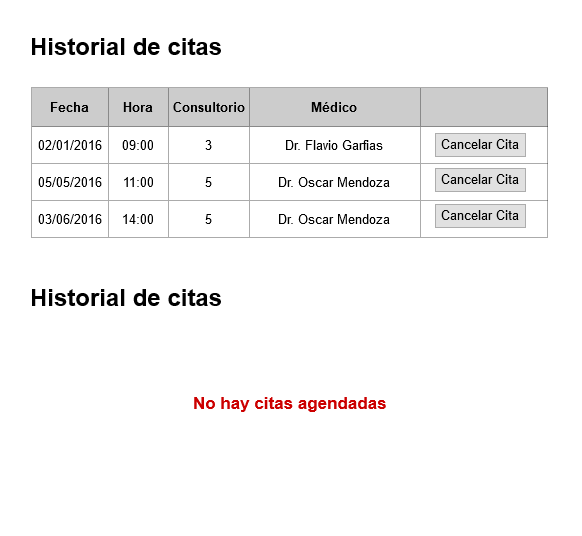
\includegraphics[width=0.8\textwidth]{images/gui/ui3_consultar_citas_paciente}
	\caption{Pantalla UI3 Consultar citas paciente}
\end{figure}

\subsubsection{Entradas}
\begin{itemize}
	\item Ninguna. 
\end{itemize}

\subsubsection{Salidas}
\begin{itemize}
	\item Lista de citas.
\end{itemize}

\subsubsection{Comandos}
\begin{itemize}
	\item \IUbutton{Cancelar cita}: Inicia CU Cancelar cita.
\end{itemize}

\subsubsection{Mensajes}
\begin{Citemize}
	\item {\bf MSG3a} ``No hay citas agendadas''.
\end{Citemize}

%--------------Consultar Pacientes------------

\subsection{IU21 Consultar Pacientes}

\subsubsection{Objetivo}
Mostrar al gerente la información básica de los pacientes registrados en el sistema.

\subsubsection{Diseño}
Esta pantalla aparece al presionar el botón ``Consultar Pacientes'' en la pantalla de inicio del Gerente.

\begin{figure}[htbp!]
	\centering
	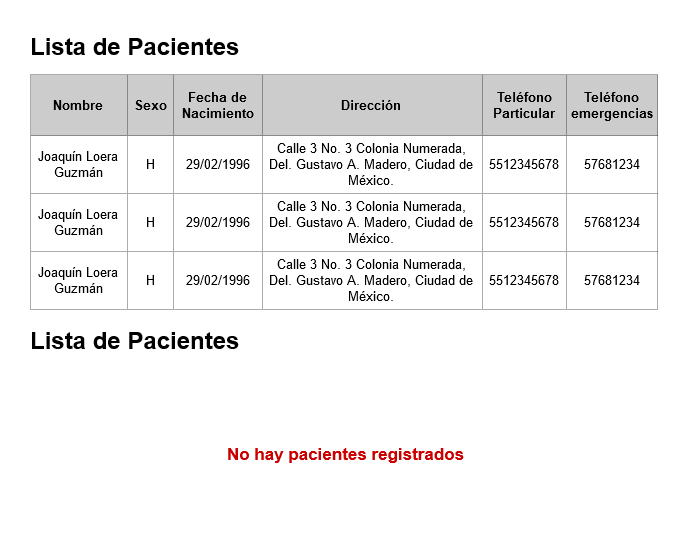
\includegraphics[width=0.8\textwidth]{images/gui/ui21_consultar_pacientes}
	\caption{Pantalla UI21 Consultar pacientes}
\end{figure}

\subsubsection{Entradas}
\begin{itemize}
	\item Ninguna.
\end{itemize}

\subsubsection{Salidas}
\begin{itemize}
	\item Lista de pacientes.
\end{itemize}

\subsubsection{Comandos}
\begin{itemize}
	\item Ninguno.
\end{itemize}

\subsubsection{Mensajes}
\begin{Citemize}
	\item {\bf MSG21a} ``No hay pacientes registrados''.
\end{Citemize}

%--------------Consultar Inventario----------------

\subsection{IU23 Consultar Inventario}

\subsubsection{Objetivo}
Mostrar al cajero la información y cantidades en inventario de los medicamentos de la farmacia.

\subsubsection{Diseño}
Esta pantalla aparece al presionar el botón ``Consultar Inventario'' en la pantalla de inicio del Cajero.

\begin{figure}[htbp!]
	\centering
	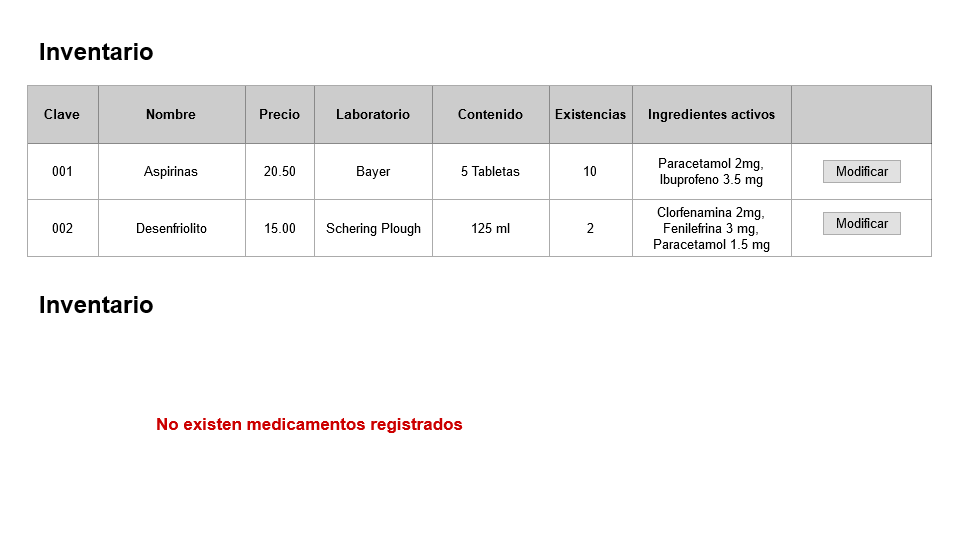
\includegraphics[width=0.8\textwidth]{images/gui/ui23_consultar_inventario}
	\caption{Pantalla UI23 Consultar inventario}
\end{figure}

\subsubsection{Entradas}
\begin{itemize}
	\item Ninguna.
\end{itemize}

\subsubsection{Salidas}
\begin{itemize}
	\item Lista de medicamentos.
\end{itemize}

\subsubsection{Comandos}
\begin{itemize}
	\item \IUbutton{Modificar} Inicia CU22 Modificar Inventario.
\end{itemize}

\subsubsection{Mensajes}
\begin{Citemize}
	\item {\bf MSG23a} ``No existen medicamentos registrados''.
\end{Citemize}

%--------------Modificar inventario---------------------


\subsection{IU22 Modificar Inventario}

\subsubsection{Objetivo}
Permitir al cajero cambiar la cantidad de existencias en almacén de un medicamento seleccionado.

\subsubsection{Diseño}
Esta pantalla aparece al presionar el botón ``Modificar'' en la pantalla IU23 Consultar Inventario.

\begin{figure}[htbp!]
	\centering
	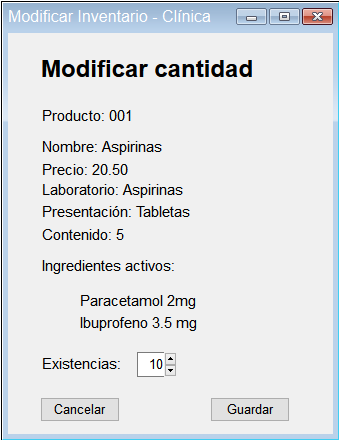
\includegraphics[width=0.5\textwidth]{images/gui/ui22_modificar_inventario}
	\caption{Pantalla UI22 Modificar inventario}
\end{figure}

\subsubsection{Entradas}
\begin{itemize}
	\item Nueva cantidad del medicamento: Entero positivo.
\end{itemize}

\subsubsection{Salidas}
\begin{itemize}
	\item Mensaje MSG22a.
\end{itemize}

\subsubsection{Comandos}
\begin{itemize}
	\item \IUbutton{Guardar} Guarda la nueva cantidad ingresada en el repositorio de datos.
	\item \IUbutton{Cancelar} Descarta los cambios realizados y muestra IU23 Consultar Inventario.
\end{itemize}

\subsubsection{Mensajes}
\begin{Citemize}
	\item {\bf MSG22a} ``Cantidad registrada correctamente''.
	\item {\bf MSG22b} ``Producto no encotrado''.
	\item {\bf MSG22c} ``Ingrese una cantidad válida''.
	\item {\bf MSG22d} ``Ingrese la cantidad''.
\end{Citemize}